\section*{Overall design}
\subsection{PIN codes}
The user will have to use PIN code to verify ownership of the smartcard via the terminal. The terminal will send this PIN + Nonce signed by its private key to the smartcard. By which the smartcard will reply with whether the PIN number is correct or not.

\subsection{Cryptography}
A certificate consisting of a public and private key will be first created on the back-end (the overall system acting as the Certificate Authority). Whenever a new smartcard is personalized, it will store the certificate of the CA, create public and private key for itself and a time-stamp of the last update of certificate revocation list which is signed by the CA certificate. Each terminal will have the same setup: CA certificate, its own public and private key, and signed time-stamp of last updated certificate revocation list.

\subsection{CA certificate stored in Terminals/Smartcards}
The main certificate from the CA stored in each terminal and smartcard is used to verify the validity and authenticity each certificate during communication. Each end point, i.e both smartcard and terminal alike, will verify the certificate of the other end point it is connecting to, whether the certificate has been revoked or not by the CA. This way when the CA has been notified of abuse or breach in one of the end points, it will only take 24 hours for each end point to know of the revocation of a particular certificate.

\subsection{Public and Private key in Terminals/Smartcards}
Public and private keys in each end point will be used in conjunction with the CA certificate to mutually authenticate between each other. It is also used to negotiate a symmetric key and also to provide integrity of the message by signing them.

\subsection{Life Cycle of Card}
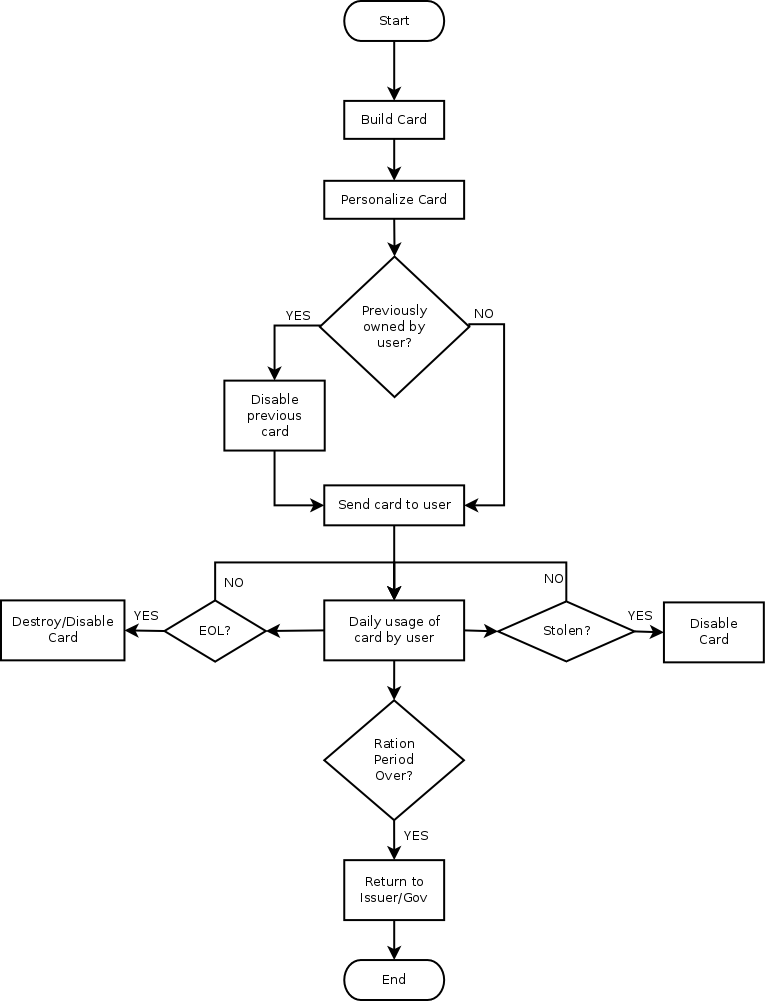
\includegraphics[width=\textwidth]{SCLifeCycle}

\subsection{Protocol Descriptions}

\subsubsection{Terminology}
	\begin{tabular}{*{2}{l}}
	 $certificate_{T}$ & certificate of Terminal \\
	 $pub_{T}$ & public key of Terminal \\
 	 $priv_{T}$ & private key of Terminal  \\
	 $IDnr_{T}$ & Identification (ID) number of Terminal \\
	 $Nonce_{T}$ & Nonce from Terminal \\
	 $SK$ & Symmetric Key \\
	 $Verify$ & Certificate Verification function \\
	 $H$ & Cryptographic Hash function \\
	 $Slog$ & Secure Logging function \\
	 $T$ & Terminal (charging/petrol) \\
	 $JC$ & JavaCard (smartcard) \\
	 $BE$ & Back-end (most closet communication to CA)\\
	 $CVR$ & Certificate Validity Request \\
	 $PIN$ & PIN number \\
	 $PIN_{AUTH}$ & True or False response based on in-/valid PIN \\
	 $C_{pt}$ & current possessed petrol points (in liters) \\
	 $A_{pt}$ & current monthly petrol allowance (in liters) \\
	 $W_{pt}$ & wanted petrol points (in liters) \\
	\end{tabular}
	
\subsubsection{Mutual Authentication}
T $\to$ JC: commandAPDU to enable applet.\\
T $\to$ JC: $certificate_{T}+pub_{T}$\\
JC: $Verify(certificate_{T})$\\
JC $\to$ T: $SK\{[H(IDnr_{JC}||Nonce_{JC})]_{priv_JC}+IDnr_{JC}+Nonce_{JC}+certificate_{JC}\}+[SK]_{pub_T}$\\
T $\to$: $Verify(certificate_{JC})$\\
T $\to$ JC: $SK\{[H(IDnr_{T}||Nonce_{T})]_{priv_T}+IDnr_{T}+Nonce_{T}\}$

\subsubsection{Certificate Validity Request}
Note: this is considered to be done via a secure communication after mutually authenticating between smartcard $\to$ terminal, terminal $\to$ backend and smartcard $\to$ backend through terminal.
\\
\\
JC $\to$ BE: $[CVR + pub_{JC}]_{pub_BE}$\\
BE $\to$ JC: $[H(validity||TS||Certs)_{priv_BE}+validity+TS+Certs]_{pub_JC}$\\

\subsubsection{PIN validation and authorisation}
Note: this is considered to be done via a secure communication after mutually authenticating each other.
\\
\\
T $\to$ JC: $SK\{[H(PIN||Nonce_{T})]_{priv_T}+PIN+Nonce_{T}\}$\\
JC $\to$ T: $SK\{[H(PIN_{AUTH}||Nonce_{JC})]_{priv_JC}+PIN_{AUTH}+Nonce_{JC}\}$\\

\subsubsection{Petrol usage}
Note: this is considered to be done via a secure communication after mutually authenticating each other.
\\
\\
JC $\to$ T: $SK\{[H(A_{pt}||C_{pt}||Nonce_{JC})]_{priv_JC}+A_{pt}+C_{pt}+Nonce_{JC}\}$\\
T $\to$ JC: $SK\{[H(W_{pt}||C_{pt}||Nonce_{T})]_{priv_T}+W_{pt}+C_{pt}+Nonce_{T}\}$\\
JC: $Slog([H(IDnr_{T}||W_{pt}||C_{pt})]_{priv_T}+IDnr_{T}+W_{pt}+C_{pt})$\\
T: $Slog([H(IDnr_{JC}||W_{pt}||C_{pt})]_{priv_JC}+IDnr_{JC}+W_{pt}+C_{pt})$\\
